\section{Parabolic p-Laplace Problem on an L-shaped Domain}
\label{sec:lshape-plaplace}

The preceding experiments considered smooth spatial settings and were useful for verifying the automated residual localisation. They did not yet provide a comparison with uniform refinement. We therefore consider the classical L-shaped domain benchmark based on \cite[Section~6.4]{ENDTMAYER202419}, together with the regularised parabolic $p$-Laplace model analysed in \cite{R6}. The example combines reduced primal regularity with goal functionals that may or may not be sensitive to the singularity.


\subsection{$p$-Laplace Problem and Goal Functional}
\label{subsec:lshape-benchmark}

Let
\[
  \Omega=(-1,1)^2\setminus\bigl([0,1]\times[-1,0]\bigr),
  \qquad Q=\Omega\times(0,1).
\]
We solve
\begin{equation}
  \partial_t u
  -\nabla\cdot\left[
    \bigl(|\nabla u|^2+\varepsilon^2\bigr)^{(p-2)/2}
    \nabla u
  \right]=f
  \quad\text{in }Q,
\end{equation}
with homogeneous Dirichlet conditions and $u(\cdot,0)=0$. Throughout this section,
\[
p=4,\qquad \varepsilon=10^{-2}.
\]
The regularisation removes the degeneracy of the diffusion law at $|\nabla u|=0$ and supplies the differentiability required by the nonlinear DWR identity \cite{R6}.




Writing $(r,\vartheta)$ for polar coordinates centred at the re-entrant corner, the manufactured solution is
\begin{equation}
 u_{\mathrm{ex}}(x,y,t)
 =\frac32(1-x^2)^2(1-y^2)^2
 r^{2/3}\sin\!\left(\frac{2\vartheta}{3}\right)\sin t .
\end{equation}
% The source term is then obtained by inserting this expression into the differential equation.
The manufactured forcing is defined in \(V^\ast\) by substituting \(u_{\mathrm{ex}}\) directly into the weak formulation.
Following \cite[Section~6.4.3]{ENDTMAYER202419}, we first consider the terminal spatial functional
\begin{equation}
  J_1(u)=\int_{\Omega}u(x,T)\,\mathrm dx,
  \label{eq:lshape-j1-terminal}
\end{equation}
with the exact value used in the computation as
\(
J_1(u_{\mathrm{ex}})
 =0.4142466902.
\)
We then consider the goal functional
\begin{equation}
  J_2(u)
  =\int_{0.5}^{0.75}\int_{\Omega_I}
  |\nabla u(x,t)|^4\,\mathrm dx\,\mathrm dt,
  \qquad
  \Omega_I=
  \left(-\frac{15}{16},-\frac{11}{16}\right)
  \times
  \left(\frac{11}{16},\frac{15}{16}\right),
  \label{eq:lshape-j2-local}
\end{equation}
which is nonlinear, spatially localised, and active only on the time window $[0.5,0.75]$. The reference value used in the computation is
\(
J_2(u_{\mathrm{ex}})=5.2366347\times10^{-5}.
\)
% High-order tensor-product Gauss quadrature applied to the analytic gradient of \eqref{eq:lshape-exact} gives

For the following experiments, the primal space is set to be $\mathrm{cG}(1) \otimes \mathrm{dG}(0)$, and both the enriched primal and adjoint use $\mathrm{cG}(2) \otimes \mathrm{dG}(1)$.
% \pef{Format spaces consistently in all examples}


\subsection{Global Terminal Goal}

Since the terminal spatial-average functional $J_1$ is global in space, it retains some sensitivity to the singularity at the re-entrant corner. The adaptive computation employs the spatial bulk parameter $\theta=0.35$ and a temporal marking fraction of $0.10$.

The computed goal error exhibits an overall decreasing trend over the six adaptive cycles,
% Its magnitude decreases from
% \(
%  |J_1(u)-J_1(u_h)|=4.699\times 10^{-3}
% \)
% on the initial discretisation to $1.21\times 10^{-3}$ at adaptive iteration~7. 
% The decrease is not strictly monotone, which is expected for a signed global quantity of interest because local space--time contributions may partially cancel after each non-uniform refinement step.
while the global effectivity is initially poor and non-monotone, but improves during the later adaptive cycles, attaining \(1.1522\) at iteration~6. \cref{fig:lshape-terminal-meshes} shows the spatial meshes associated with four representative time slabs from the adaptive sequence. Although the primal solution has reduced regularity at the re-entrant corner for \(t>0\), the local DWR indicators depend on the interaction between the primal residual and the adjoint sensitivity. Since \(J_1\) acts only at \(t=T\), the adjoint information is introduced at the terminal time and becomes spatially smoother as it is propagated backwards. These features provide an explanation for the pronounced corner refinement in the terminal slab and the absence of comparable concentration in the earlier slabwise meshes.

\cref{fig:lshape-terminal-meshes} shows a clear change in the spatial distribution of refinement across the time slabs. At \(t=0.5\) and \(t=0.75\), refinement is distributed over a broader region in the upper part of the domain, whereas the final slab exhibits a pronounced concentration near the re-entrant corner. Unlike the preceding slabs, the final slab contains the direct terminal contribution \(J_1'(u_h)(e_u(T))\). This term weights the terminal primal approximation error, which is particularly significant near the re-entrant corner because of the reduced spatial regularity. In the earlier slabs this direct terminal contribution is absent, and the indicators instead reflect the combined effect of the slab residuals and the backward-propagated adjoint weights, resulting in a more distributed pattern.

% Each local DWR indicator contains residual information weighted by the corresponding primal or dual enrichment error. For the present \(\mathrm{cG}(1)\otimes\mathrm{dG}(0)\) approximation, the discrete time derivative vanishes within each slab and the discrete nonlinear flux is constant on each spatial cell. Its action against an interior cell-bubble test therefore has no cell-interior contribution, so the cell-volume recovery is driven by the manufactured right-hand side in its weak form. Writing \(u_{\mathrm{ex}}(x,t)=\phi(x)\sin t\), this action is
% \[
% \begin{aligned}
% \langle f(t),v\rangle
% ={}&(\phi\cos t,v)
% +\sin^3t\bigl(|\nabla\phi|^2\nabla\phi,\nabla v\bigr)\\
% &+\varepsilon^2\sin t(\nabla\phi,\nabla v).
% \end{aligned}
% \]
% The bounded first contribution decreases over \(t\in[0,1]\), and its spatial factor \(\phi\) is largest along the upper-left diagonal at a moderate distance from the corner. In contrast, the leading nonlinear flux contribution carries the singular gradient of \(\phi\) and becomes relatively more important towards \(t=T\). For reference, the temporal ratio \(\sin^3t/\cos t\) increases from \(0.13\) at \(t=0.5\) to \(0.43\) at \(t=0.75\) and \(1.10\) at \(t=1\); since the associated spatial factors differ, these values describe only the relative temporal trend.

\begin{figure}[h]
  \centering
  \begin{subfigure}[t]{0.24\textwidth}
    \centering
    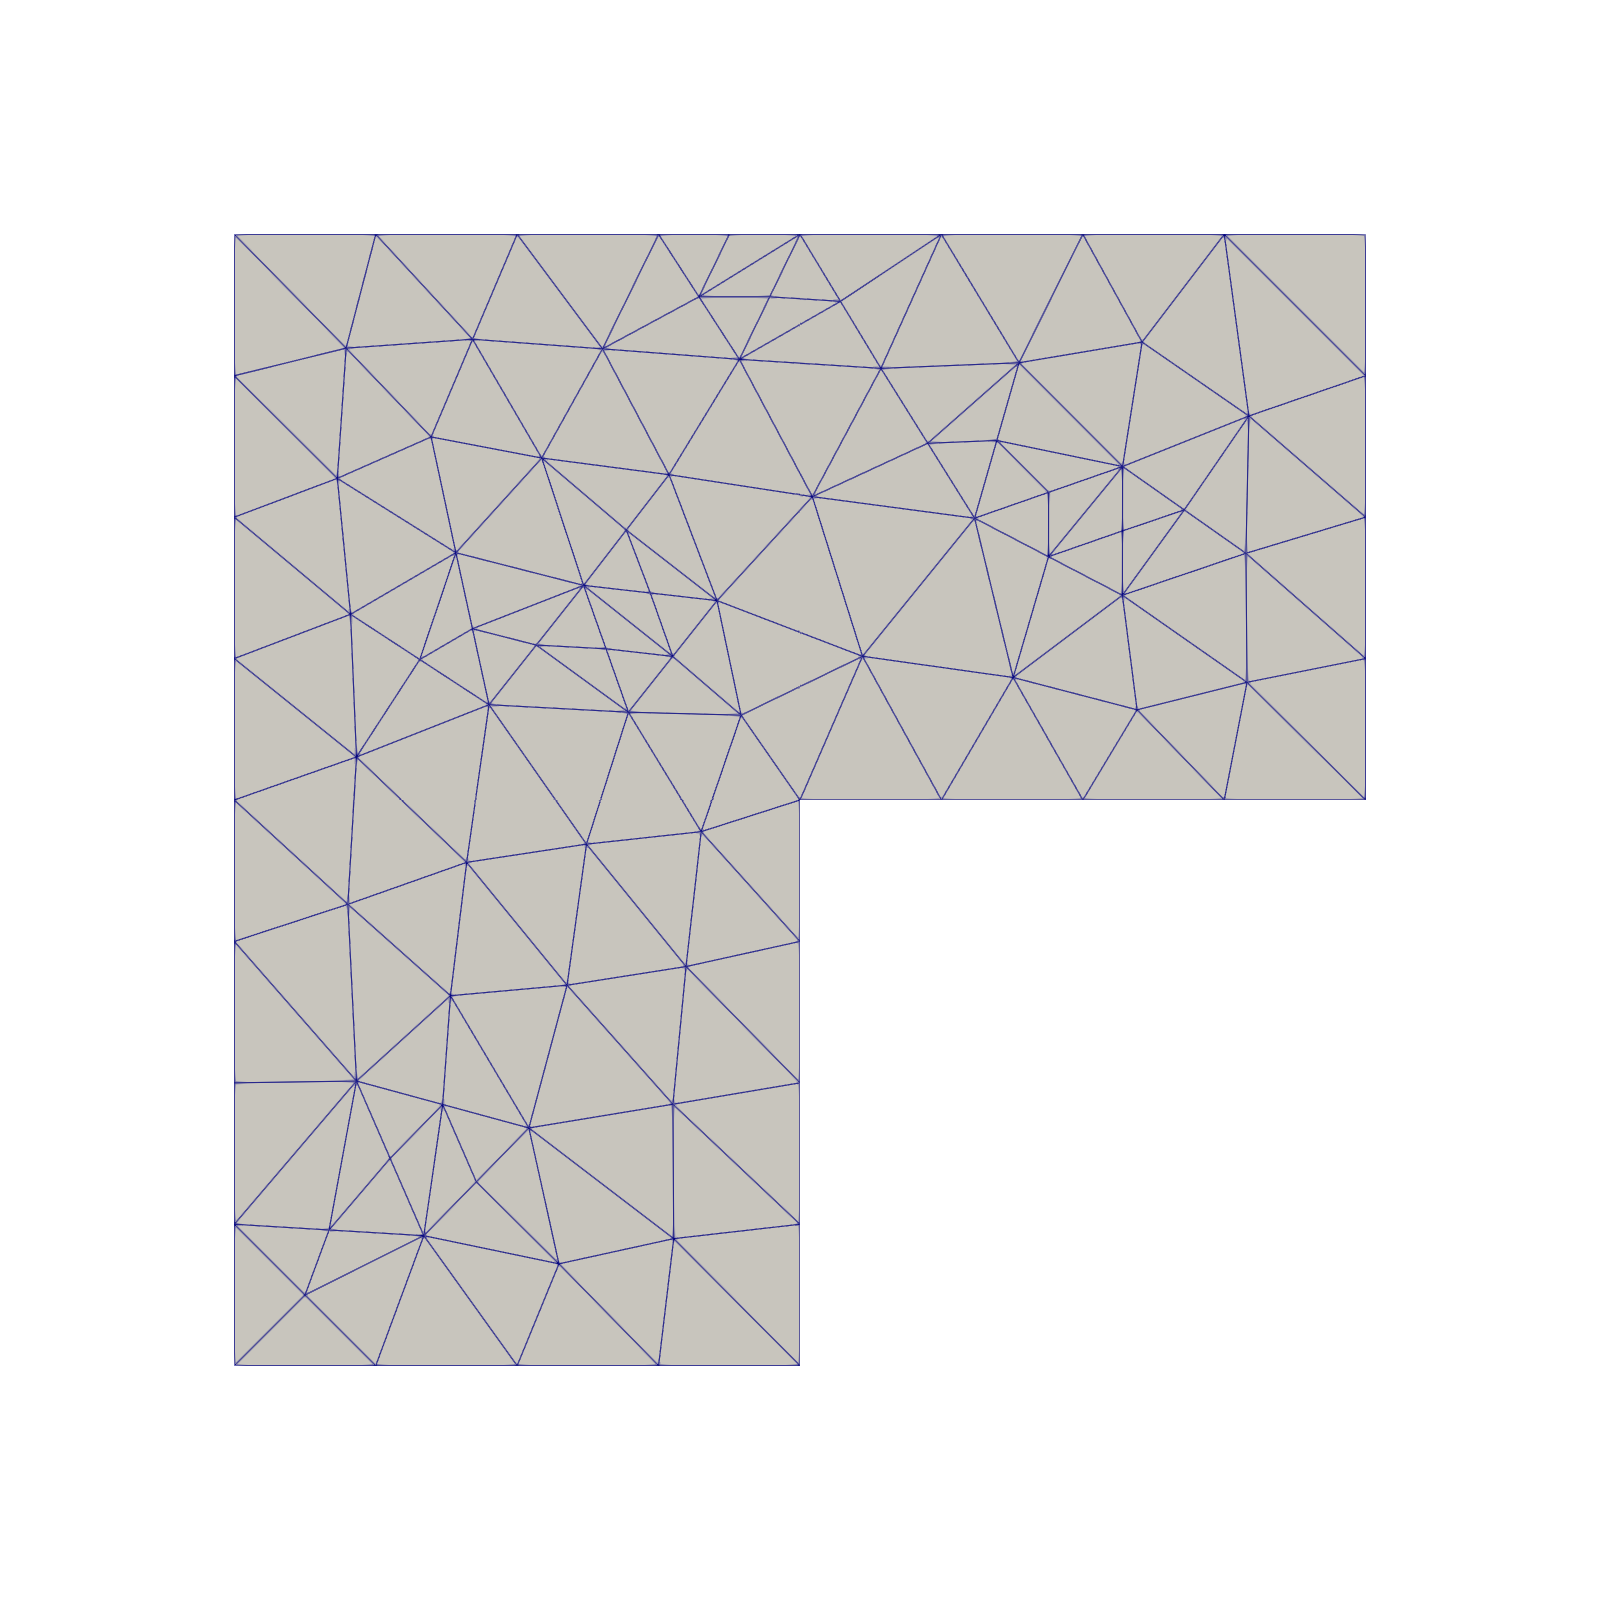
\includegraphics[width=\linewidth]
      {figures/lshape/j2_mesh.0000.png}
    \caption{$t=0$}
  \end{subfigure}
  \hfill
  \begin{subfigure}[t]{0.24\textwidth}
    \centering
    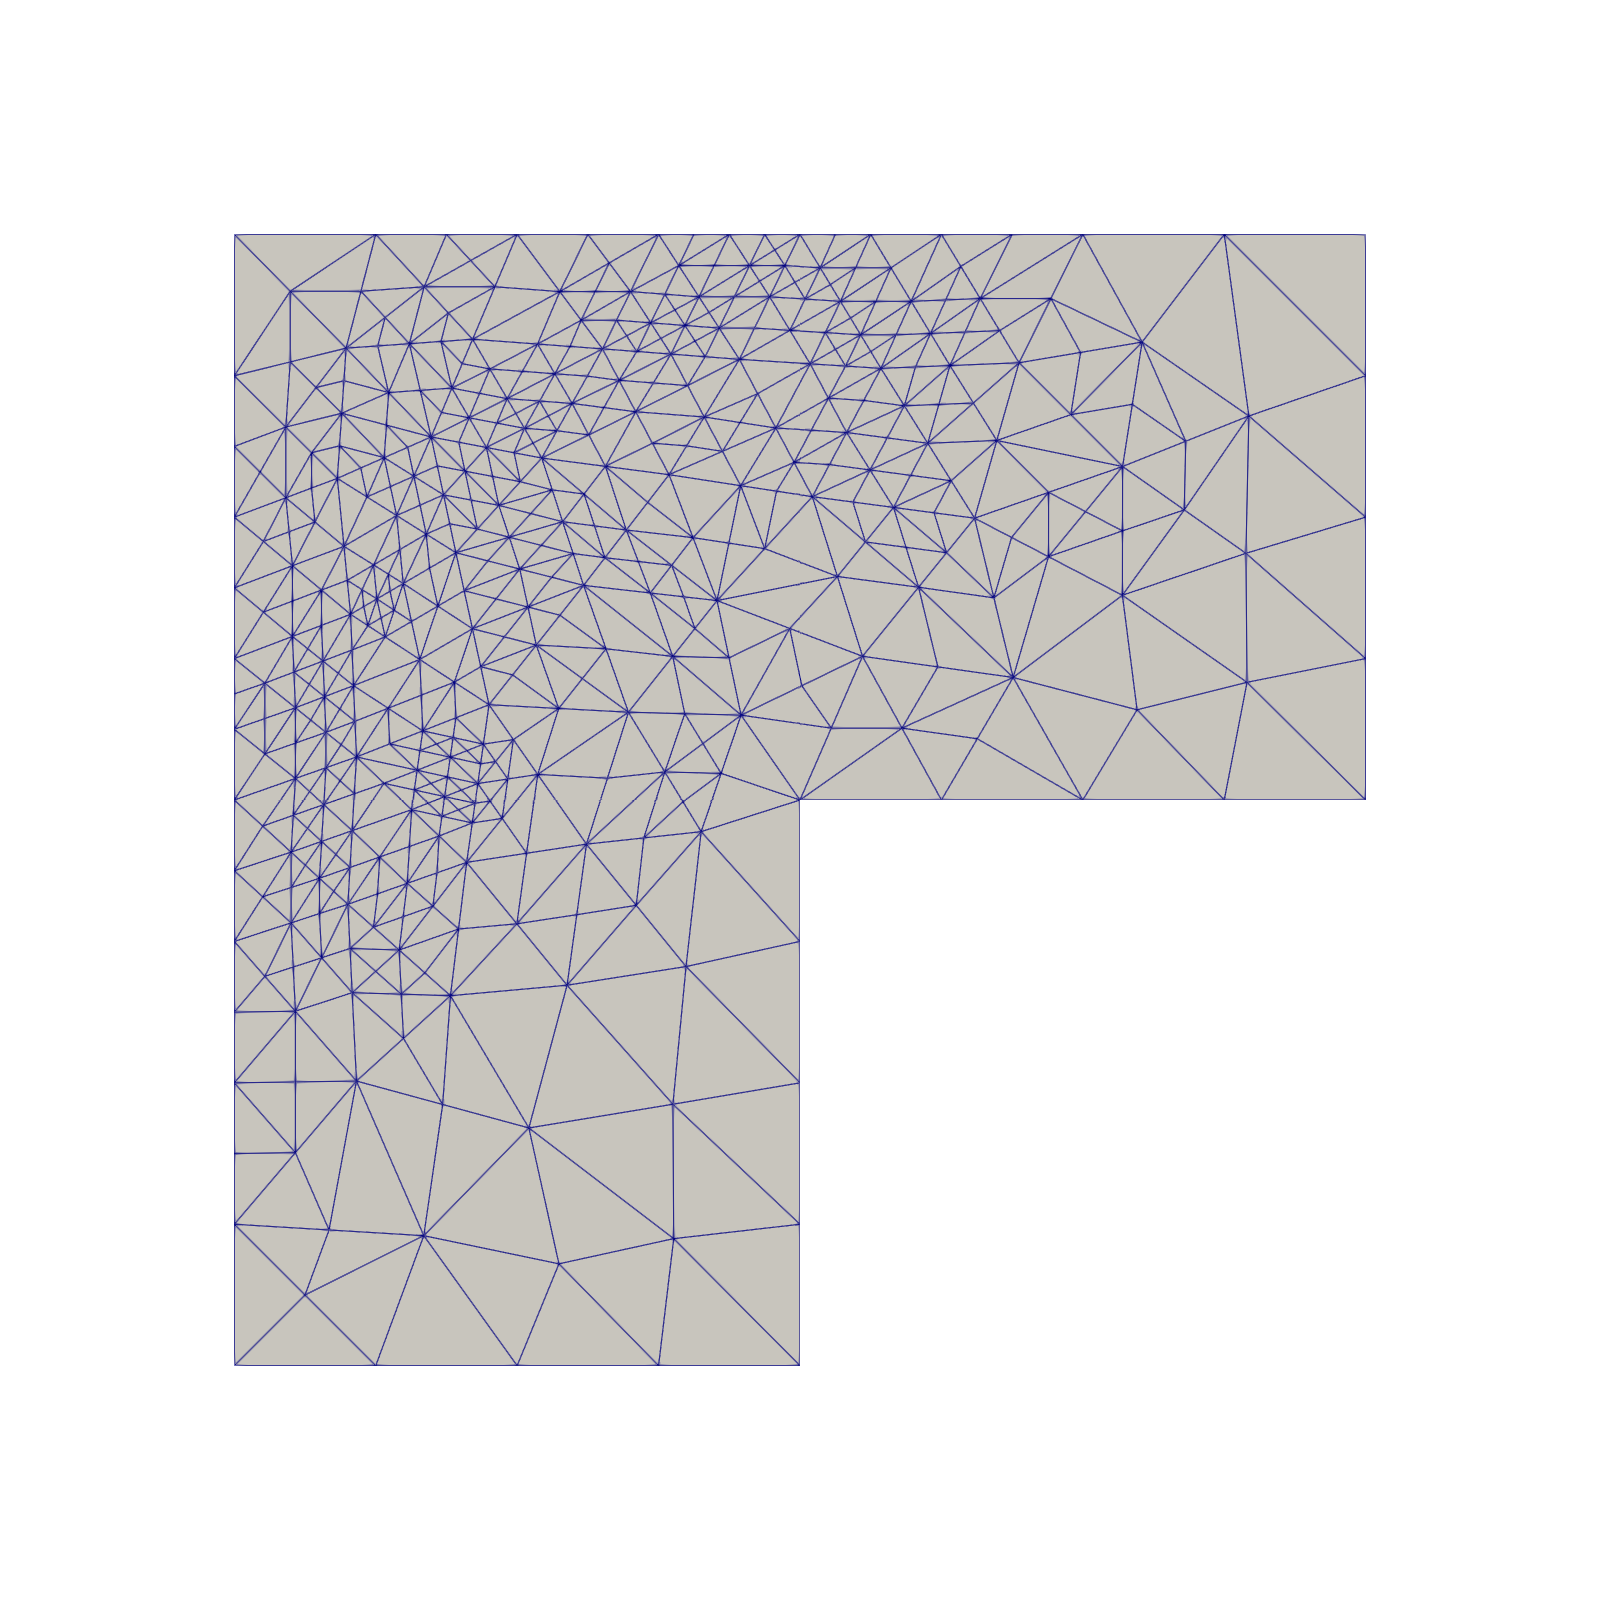
\includegraphics[width=\linewidth]
      {figures/lshape/j2_mesh.0001.png}
    \caption{$t=0.5$}
  \end{subfigure}
  \hfill
  \begin{subfigure}[t]{0.24\textwidth}
    \centering
    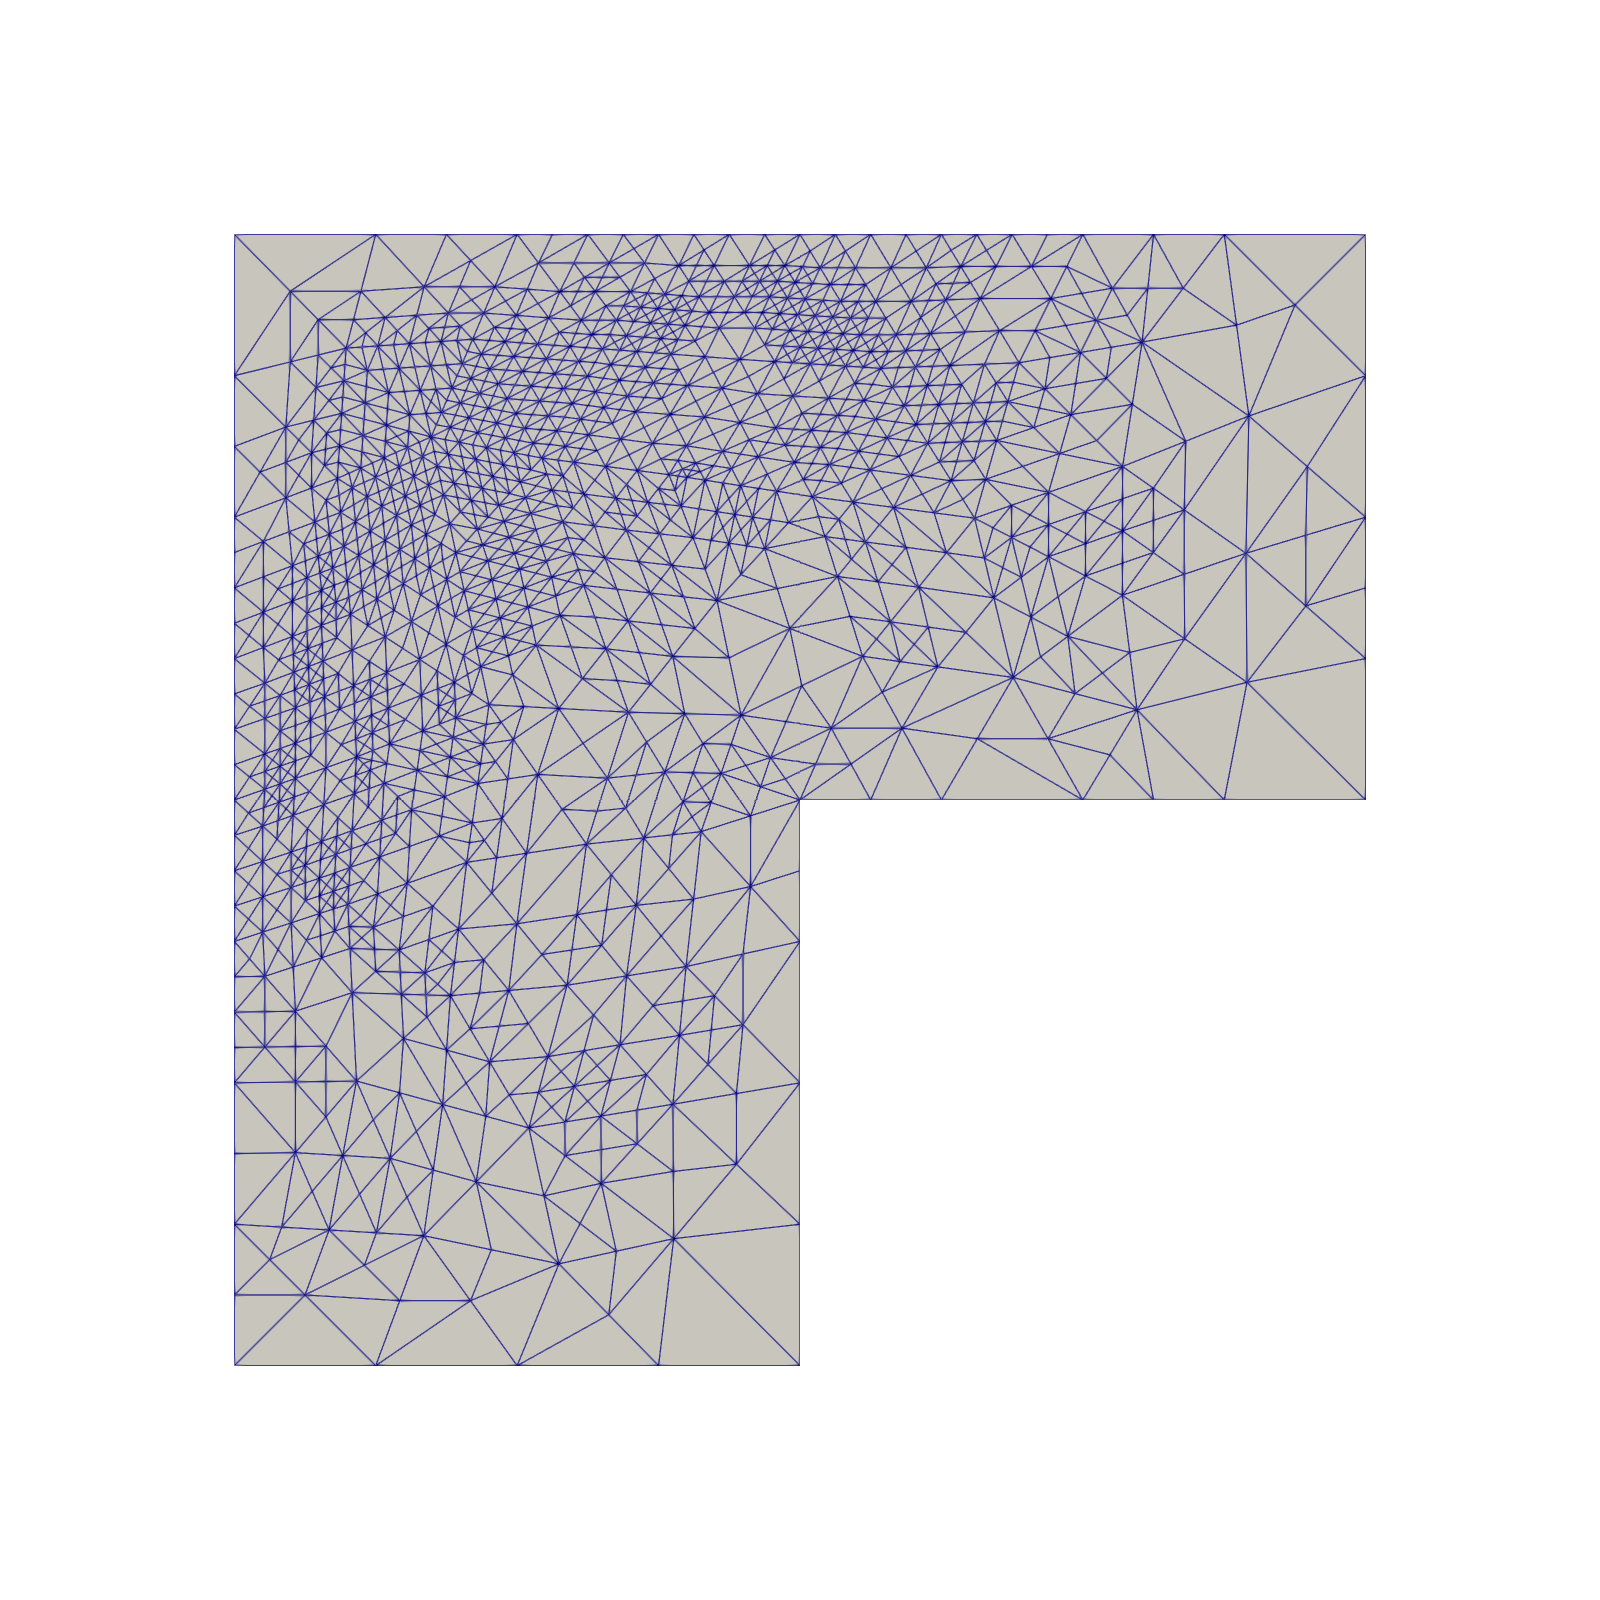
\includegraphics[width=\linewidth]
      {figures/lshape/j2_mesh.0002.png}
    \caption{$t=0.75$}
  \end{subfigure}
  \hfill
  \begin{subfigure}[t]{0.24\textwidth}
    \centering
    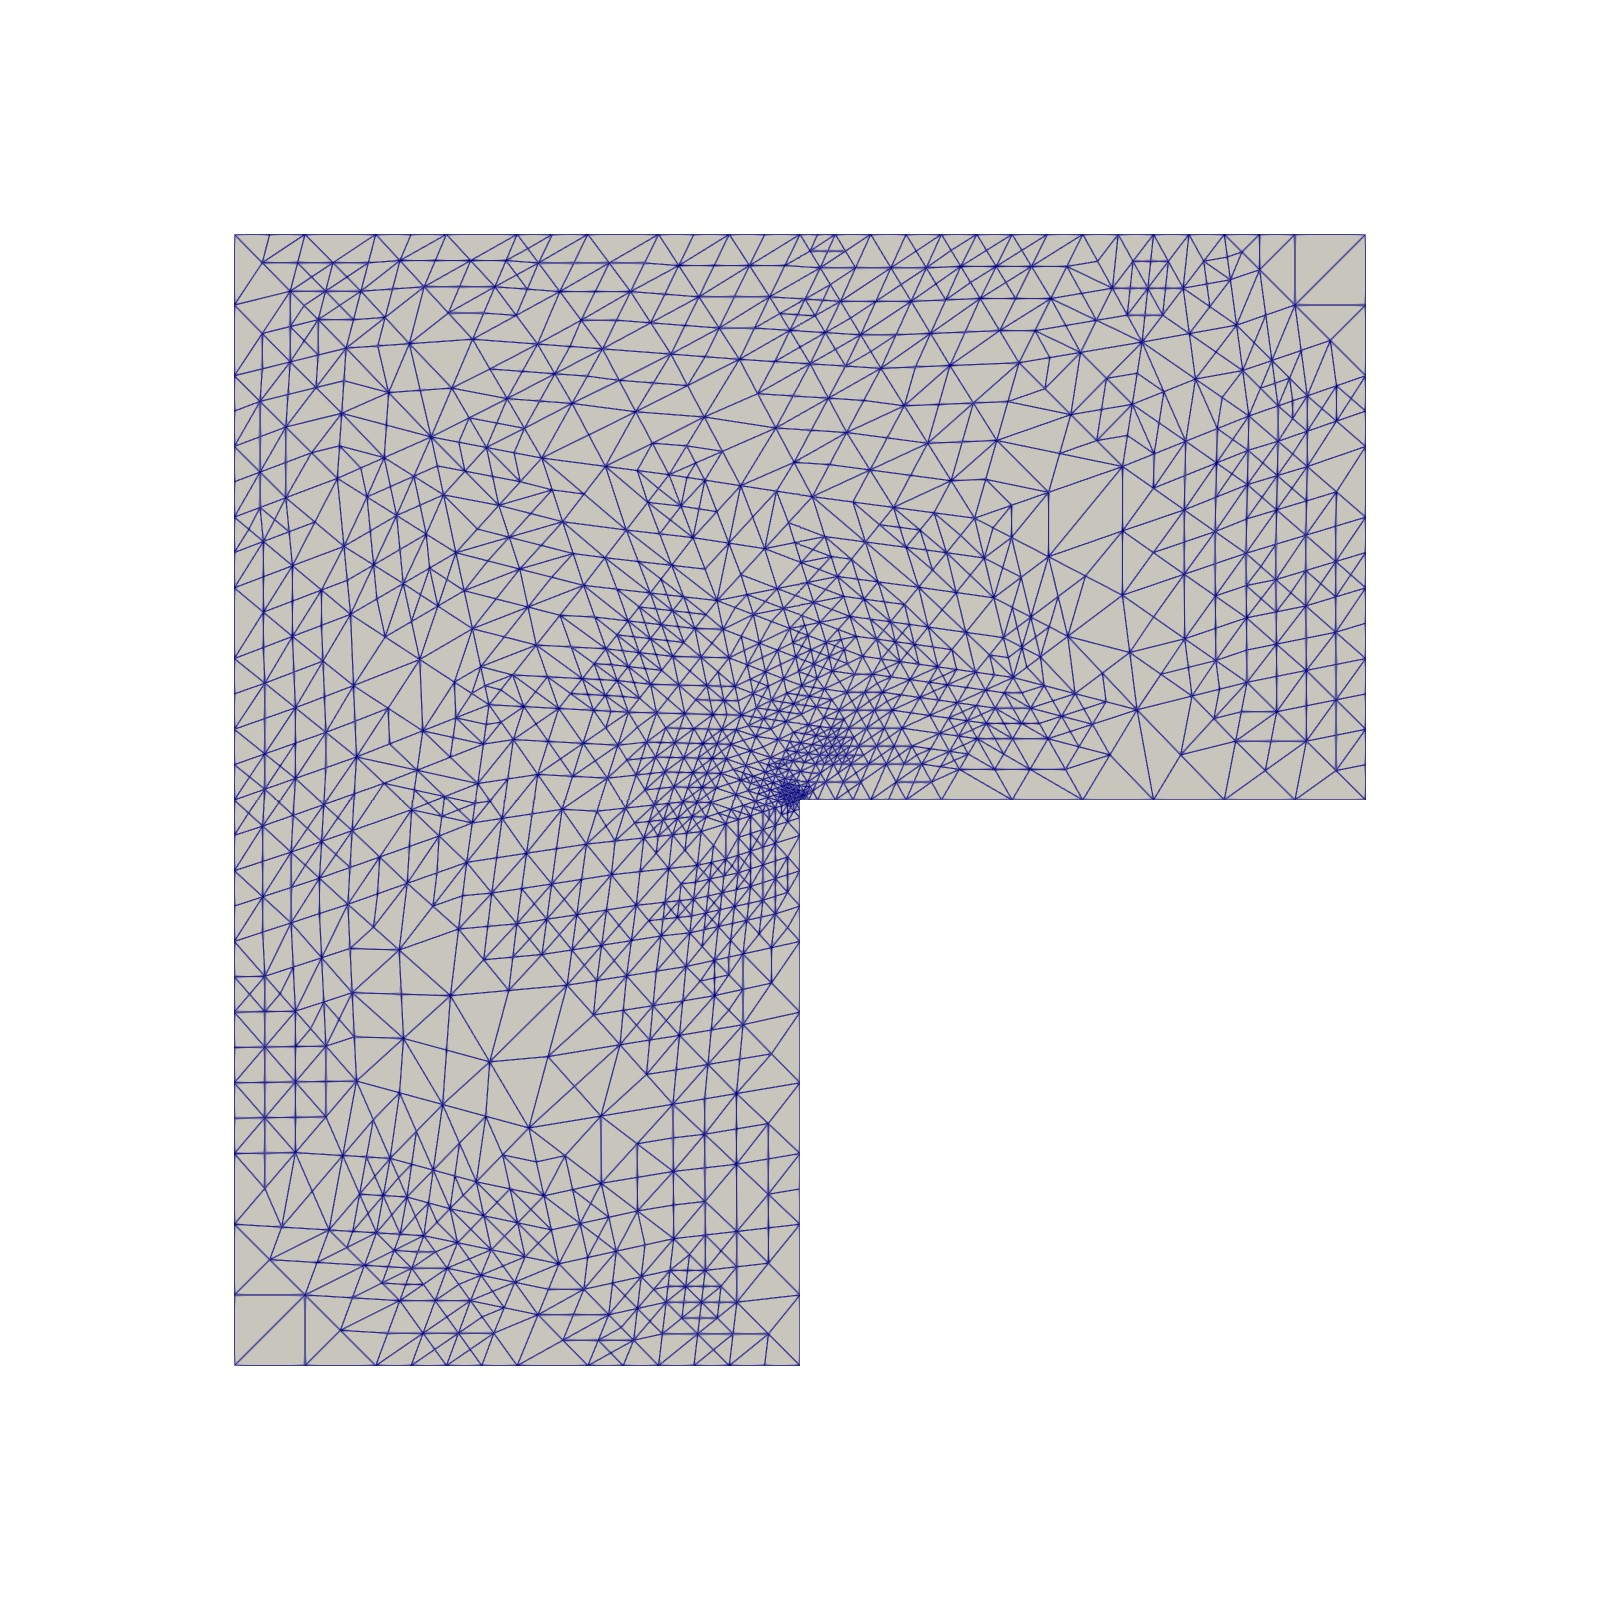
\includegraphics[width=\linewidth]
      {figures/lshape/j2_mesh.0003.png}
    \caption{$t=1$}
  \end{subfigure}
  \caption{Spatial meshes at time $t=0,\,0.5,\,0.75,\,1$ for goal $J_1$ at iteration~6.}
  \label{fig:lshape-terminal-meshes}
\end{figure}


\subsection{Localised Nonlinear Goal}

For the goal functional \(J_2\), the observation rectangle
\(
\Omega_I
=
\left(-\frac{15}{16},-\frac{11}{16}\right)
\times
\left(\frac{11}{16},\frac{15}{16}\right)
\)
is represented as a separate \texttt{Netgen} material subdomain, so that its boundary consists of mesh facets. The initial discretisation contains eight time slabs and uses the fitted mesh with \(75\) terminal spatial degrees of freedom. For the adaptive run, the D\"orfler marking fraction is set to \(\theta=0.30\). A slab is bisected when at least \(10\%\) of its cells have been selected by the global marking step. The uniform run refines every spatial cell and bisects every time slab. Both runs start from the same space--time discretisation.

\cref{fig:lshape-j2-comparison} compares the true \(J_2\) error against
\(
N_{\mathrm{st}}
=
\sum_{n=1}^{N_t}\dim V_h^n,
\)
which counts the actual slabwise primal unknowns. The errors and global effectivity indices at representative iterates are reported in~\cref{tab:lshape-j2-results}.

\begin{figure}[h]
  \centering
  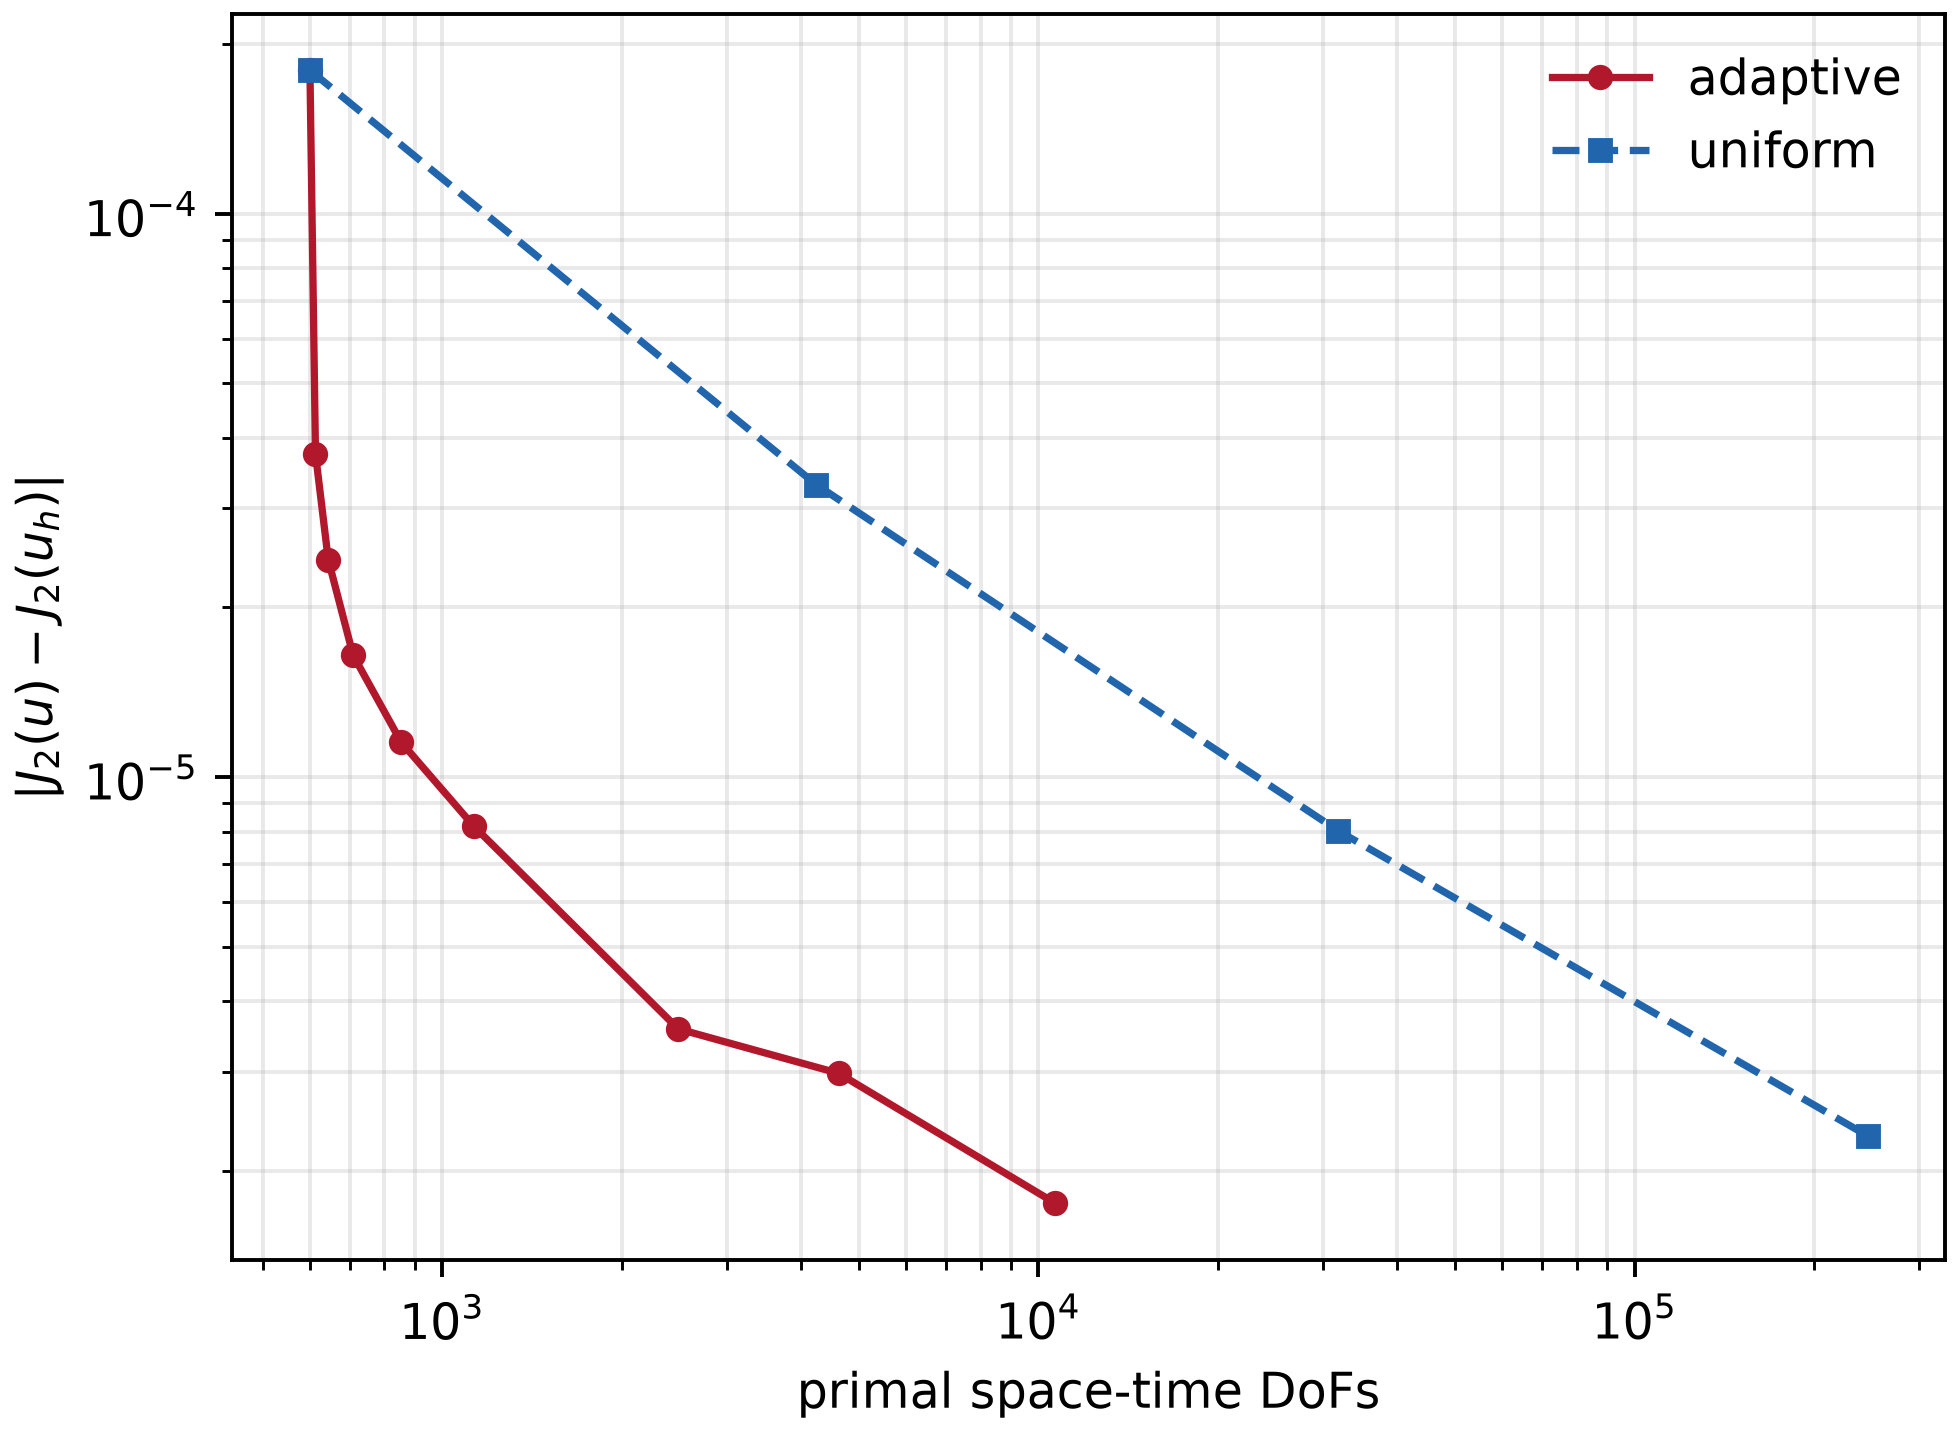
\includegraphics[width=0.65\textwidth]
  {figures/lshape/plaplace_windowed_adaptive_uniform.png}
  \caption{\(J_2\) error against total primal space--time degrees of freedom for adaptive iterations \(0\)--\(8\) and uniform iterations \(0\)--\(3\).}
  \label{fig:lshape-j2-comparison}
\end{figure}

\begin{table}[htbp]
\centering
\small
\setlength{\tabcolsep}{4pt}
\begin{tabular}{lrrrrrr}
\toprule
Strategy/iter.
& \(N_{\mathrm{st}}\)
& \(N_{\mathrm{cell}}\)
& \(N_t\)
& \(\lvert J_2(u)-J_2(u_h)\rvert\)
& \(\eta_{\mathrm{global}}\)
& \(I_{\mathrm{eff}}^{\mathrm{glob}}\) \\
\midrule
uniform 1
& \(4\,240\)
& \(7\,424\)
& \(16\)
& \(3.3043\times10^{-5}\)
& \(-3.5743\times10^{-5}\)
& \(1.0817\) \\

uniform 2
& \(31\,776\)
& \(59\,392\)
& \(32\)
& \(8.0353\times10^{-6}\)
& \(-8.2195\times10^{-6}\)
& \(1.0229\) \\

uniform 3
& \(245\,824\)
& \(475\,136\)
& \(64\)
& \(2.3074\times10^{-6}\)
& \(-2.3238\times10^{-6}\)
& \(1.0071\) \\

\midrule
adaptive 2
& \(644\)
& \(1\,016\)
& \(8\)
& \(2.4307\times10^{-5}\)
& \(-2.6793\times10^{-5}\)
& \(1.1023\) \\

adaptive 4
& \(854\)
& \(1\,431\)
& \(8\)
& \(1.1522\times10^{-5}\)
& \(-1.2089\times10^{-5}\)
& \(1.0492\) \\

adaptive 6
& \(2\,488\)
& \(4\,587\)
& \(10\)
& \(3.5721\times10^{-6}\)
& \(-3.6541\times10^{-6}\)
& \(1.0229\) \\

adaptive 8
& \(10\,654\)
& \(20\,514\)
& \(17\)
& \(1.7536\times10^{-6}\)
& \(-1.7838\times10^{-6}\)
& \(1.0172\) \\
\bottomrule
\end{tabular}
\caption{Selected uniform and adaptive results for the localised nonlinear goal \(J_2\).}
\label{tab:lshape-j2-results}
\end{table}

The adaptive sequence reduces the goal error considerably more efficiently than uniform refinement. At adaptive iteration \(8\), it attains an error of \(1.7536\times10^{-6}\) using \(10\,654\) primal space--time degrees of freedom. By comparison, uniform iteration \(3\) uses \(245\,824\) degrees of freedom to obtain the larger error \(2.3074\times10^{-6}\). Uniform refinement therefore requires approximately \(23.1\) times as many primal space--time degrees of freedom while its final goal error is approximately \(24\%\) larger. The global effectivity indices in the selected adaptive iterations approach to one, from \(1.1023\) to \(1.0172\).

% The adaptive sequence reduces the error much more rapidly than uniform refinement. Uniform refinement uses approximately $245824/2871\simeq 85.6$ times as many primal space--time degrees of freedom to reach a comparable goal accuracy. 
% At the initial level the global and localised estimates are $-1.6628\times10^{-4}$ and $-1.6645\times10^{-4}$, giving effectivities $0.925$ and $0.926$, respectively. Uniform refinement subsequently drives both indices smoothly towards one. The adaptive global index remains between $0.925$ and $1.321$ through iterate~6, despite changing only a small fraction of the space--time cells.

% However, from the table, an unexpected decrease to $I_{\mathrm{eff}}^{\mathrm{glob}}=0.550$ occurs at adaptive iterate~7. The available reference goal value shows that this is associated with a failure of the saturation property underlying the DWR reliability and efficiency theory \cite{ENDTMAYER202419}. With $u_h^+$ denoting the enriched primal solution, the observed ratio 
% \begin{equation*}
%   b_h^{\mathrm{obs}}
%   \coloneqq\frac{|J_1(u)-J_1(u_h^+)|}{|J_1(u)-J_1(u_h)|}
%   \label{eq:lshape-observed-saturation}
% \end{equation*}
% equals $0.1296<1$ at iterate~6, where the enriched approximation is clearly more accurate, but increases to $1.382>1$ at iterate~7. At the latter level the low-order goal error has crossed zero and has the very small magnitude $1.561\times10^{-7}$, whereas the enriched goal lies on the opposite side of the exact value with error $2.157\times10^{-7}$. Enrichment no longer reduces the goal error, and the saturation-based estimate is not guaranteed. This suggested that the enriched problem should be strengthened, for example by increasing its spatial or temporal polynomial degree, if further accuracy is required.

% \yue{does this make sense? though Ieff is incorrect but the error is indeed decreasing}
% \pef{It is somewhat surprising, I think this is the first time I have seen the saturation assumption fail!}
% \yue{the goal error increases from ite. 6 to 7. I excluded ite 7 in Fig 3.10 for now, but I don't know how to explain this}

Finally, \cref{fig:lshape-j1-meshes} show the two-dimensional adapted meshes at different times.
\begin{figure}[!h]
  \centering
  \begin{subfigure}[t]{0.31\textwidth}
    \centering
    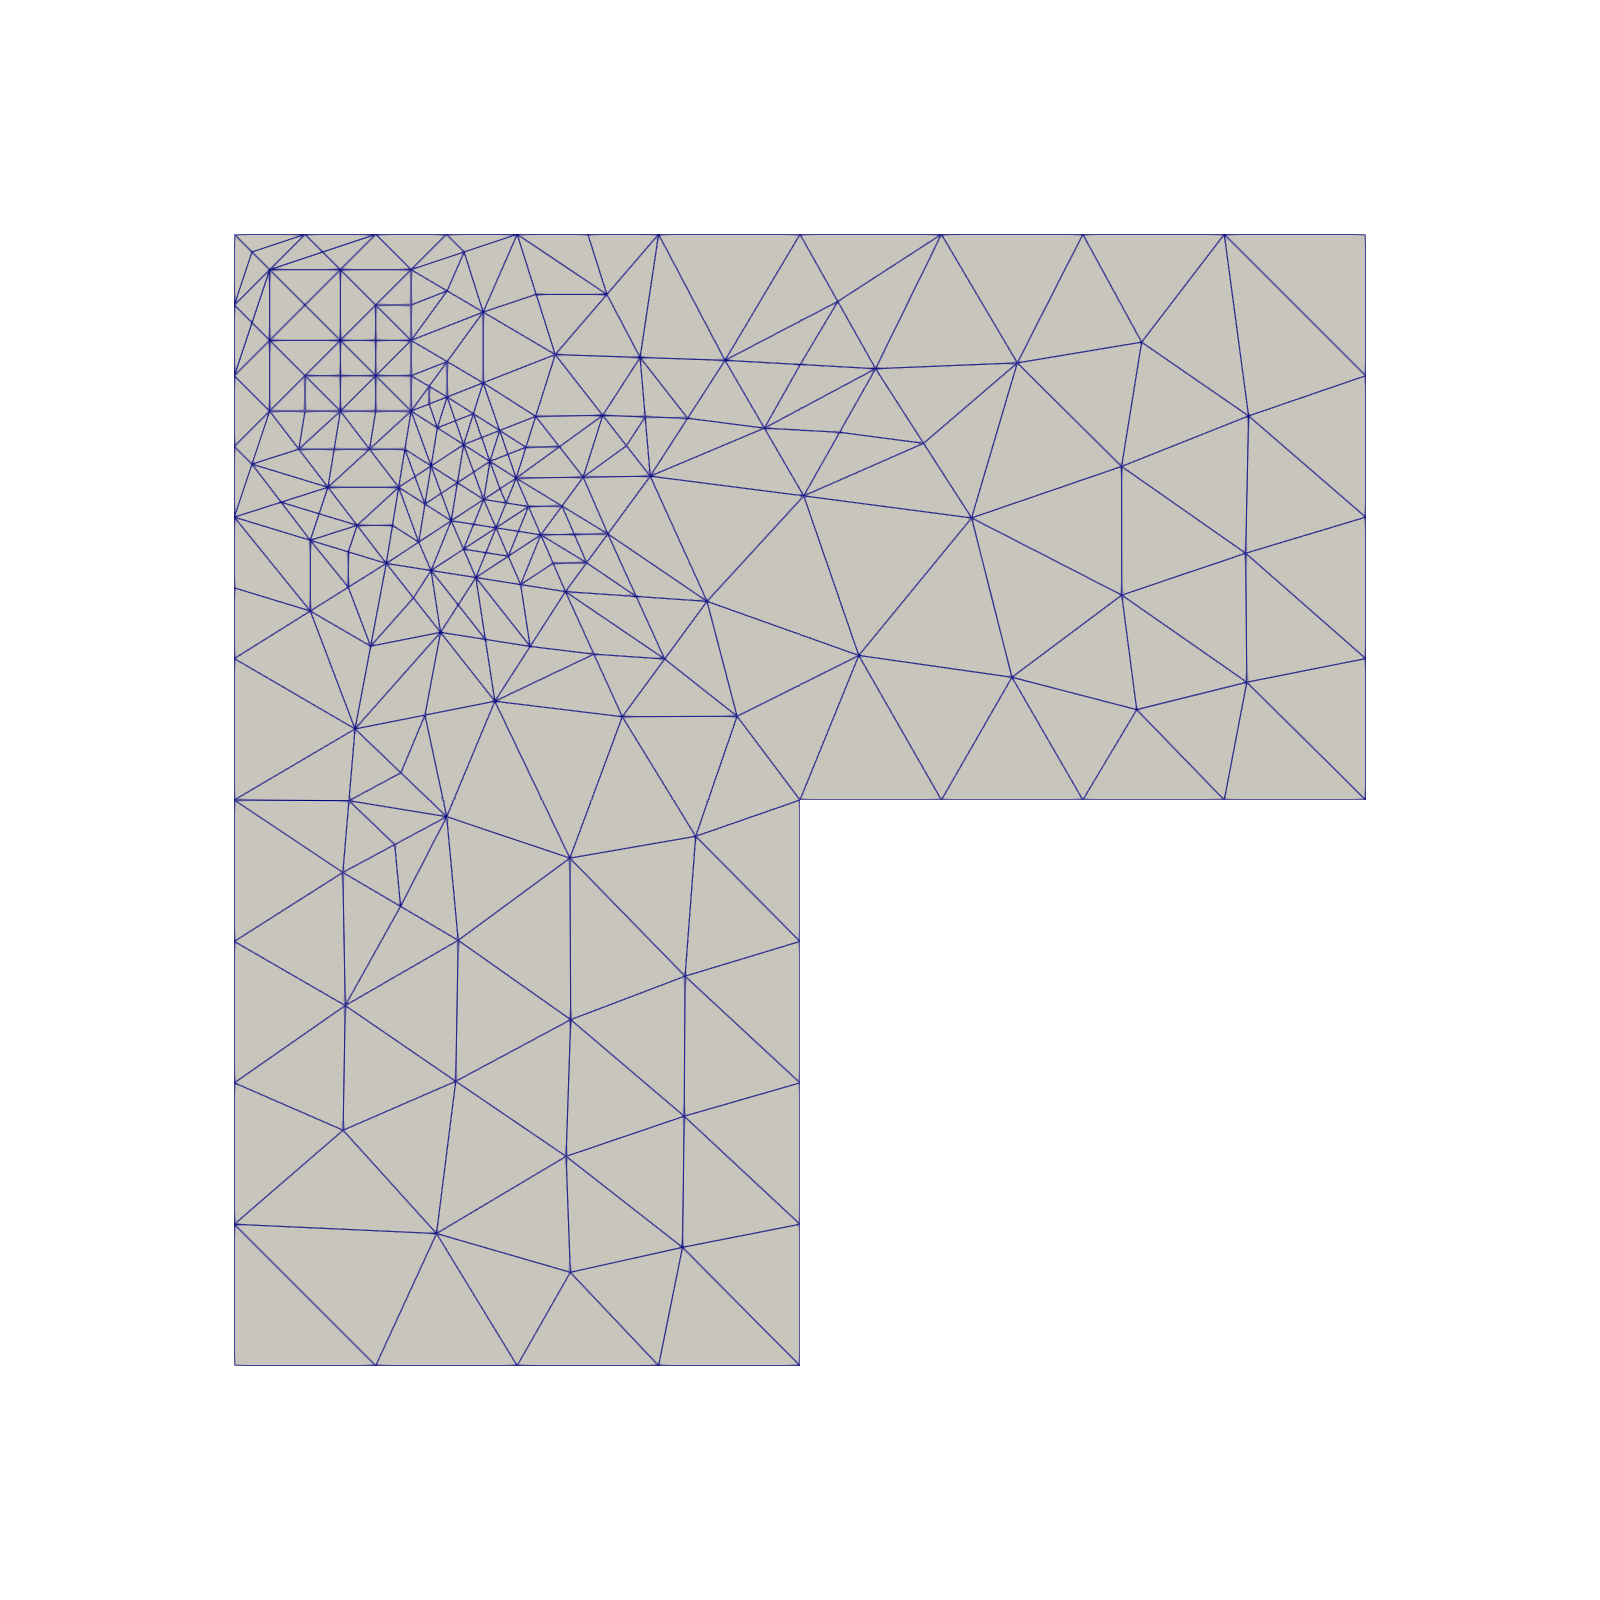
\includegraphics[
      width=\linewidth]{figures/lshape/j1_mesh.0000.png}
    \caption{}
  \end{subfigure}
  % \hfill
  \begin{subfigure}[t]{0.31\textwidth}
    \centering
    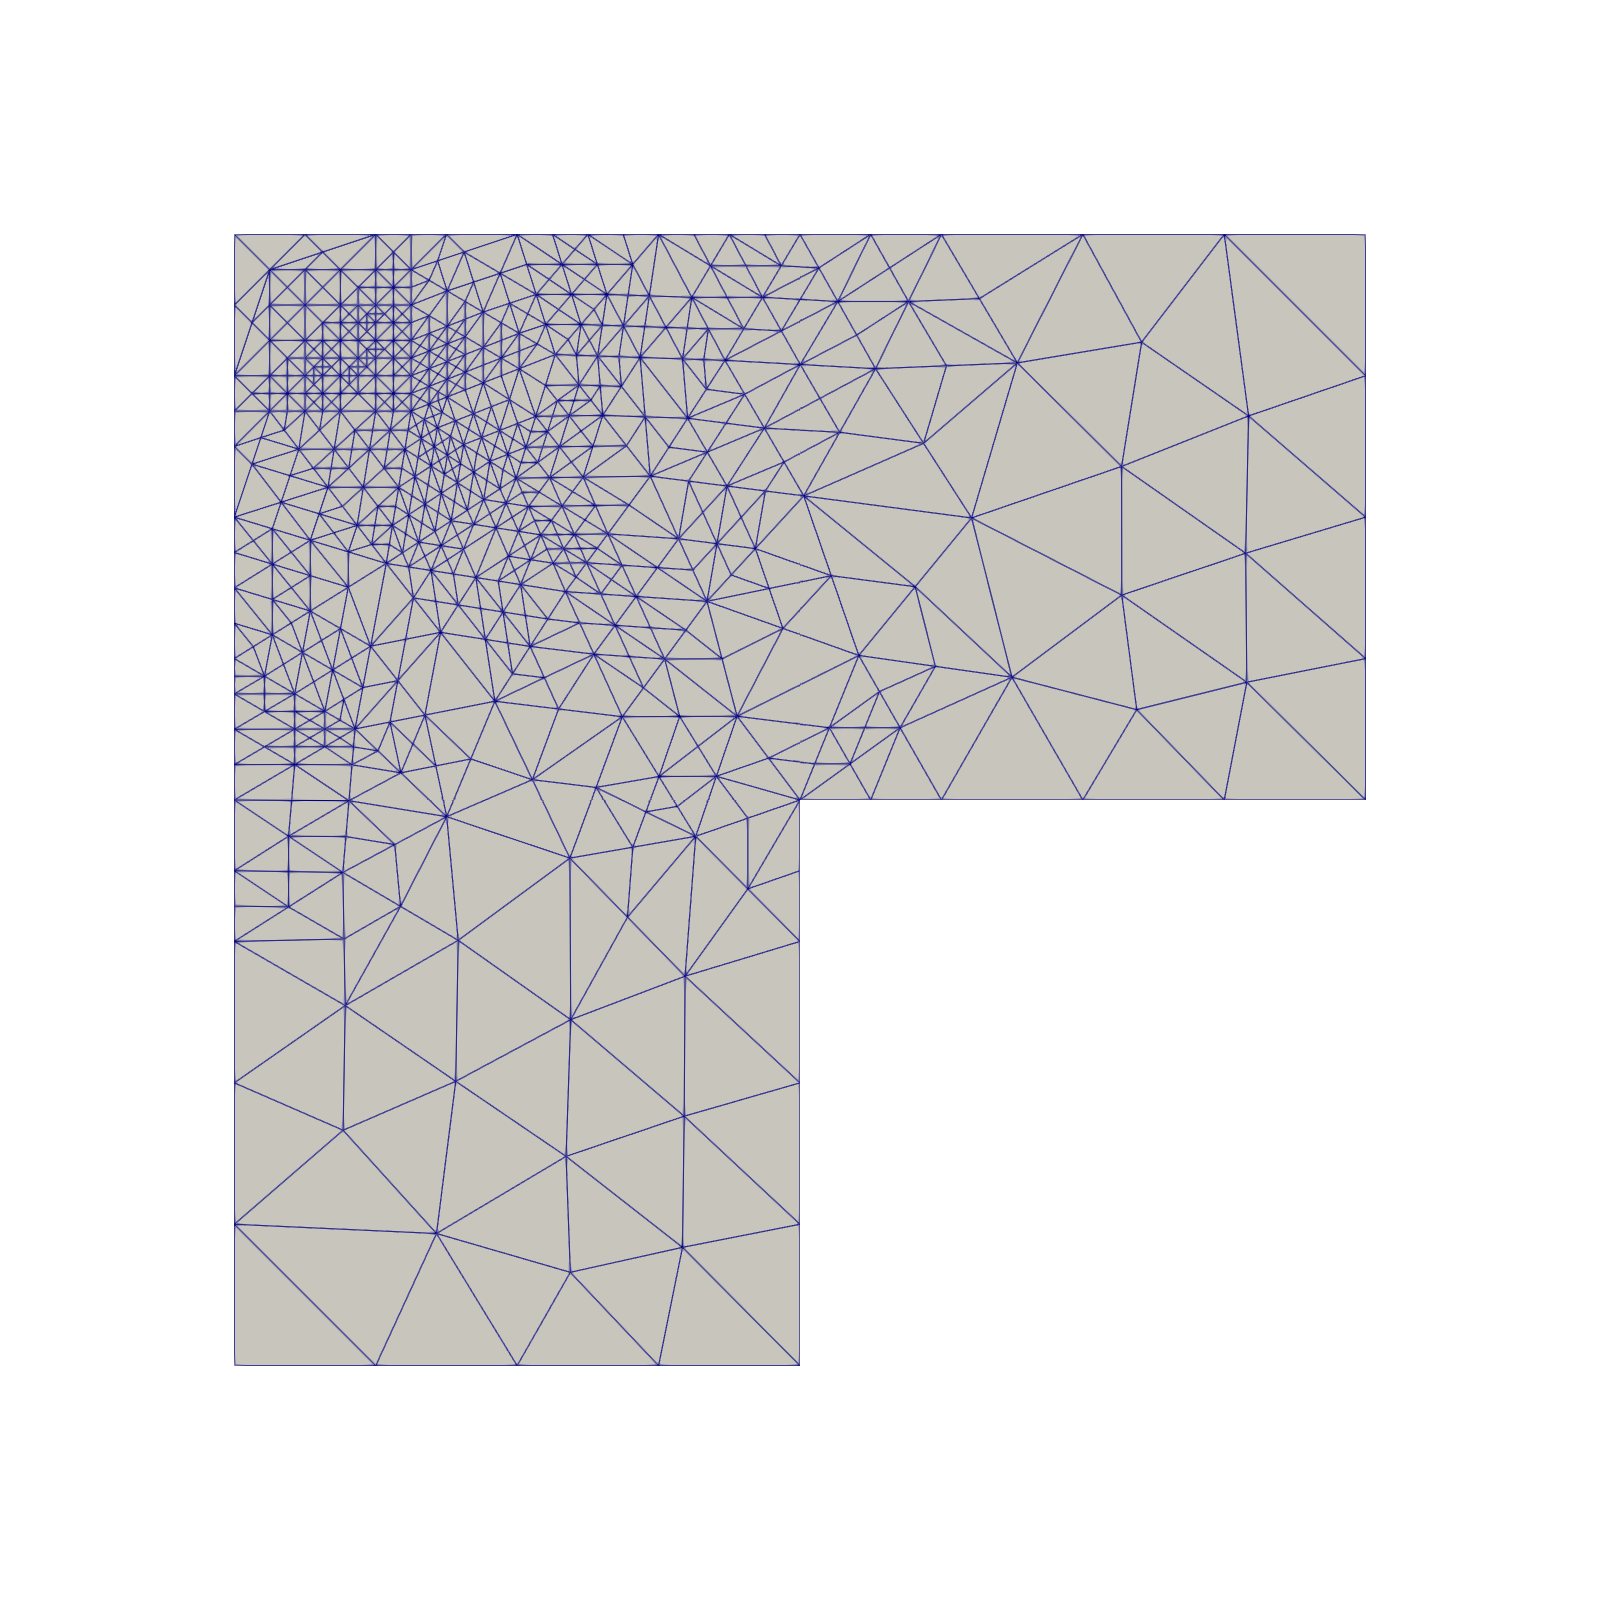
\includegraphics[
      width=\linewidth
    ]{figures/lshape/j1_mesh.0001.png}
    \caption{}
  \end{subfigure}
  \newline
  % \hfill
  \begin{subfigure}[t]{0.31\textwidth}
    \centering
    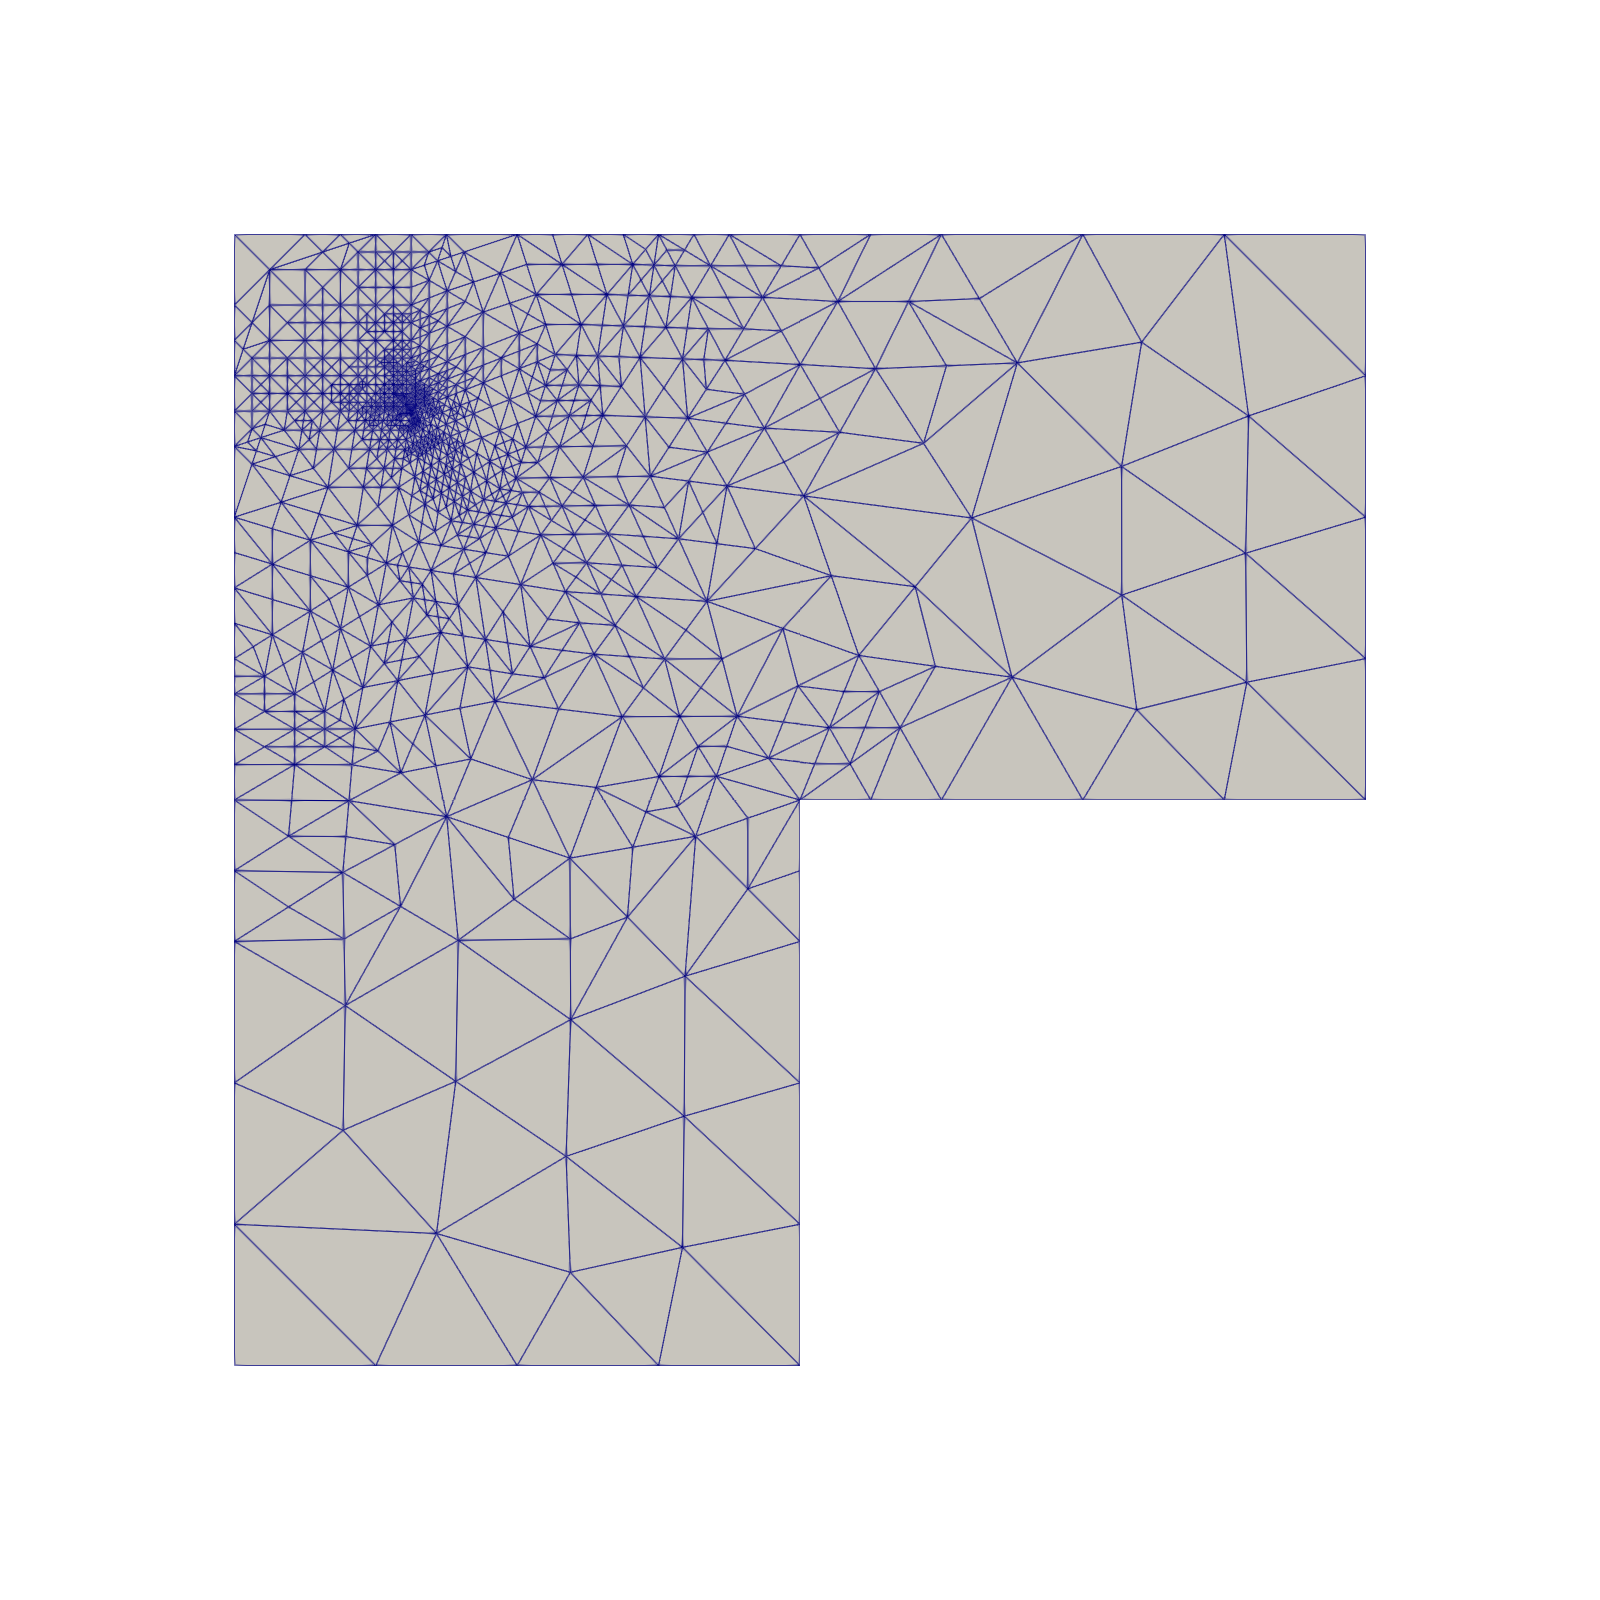
\includegraphics[
      width=\linewidth
    ]{figures/lshape/j1_mesh.0002.png}
    \caption{}
  \end{subfigure}
  \hfill
  \begin{subfigure}[t]{0.31\textwidth}
    \centering
    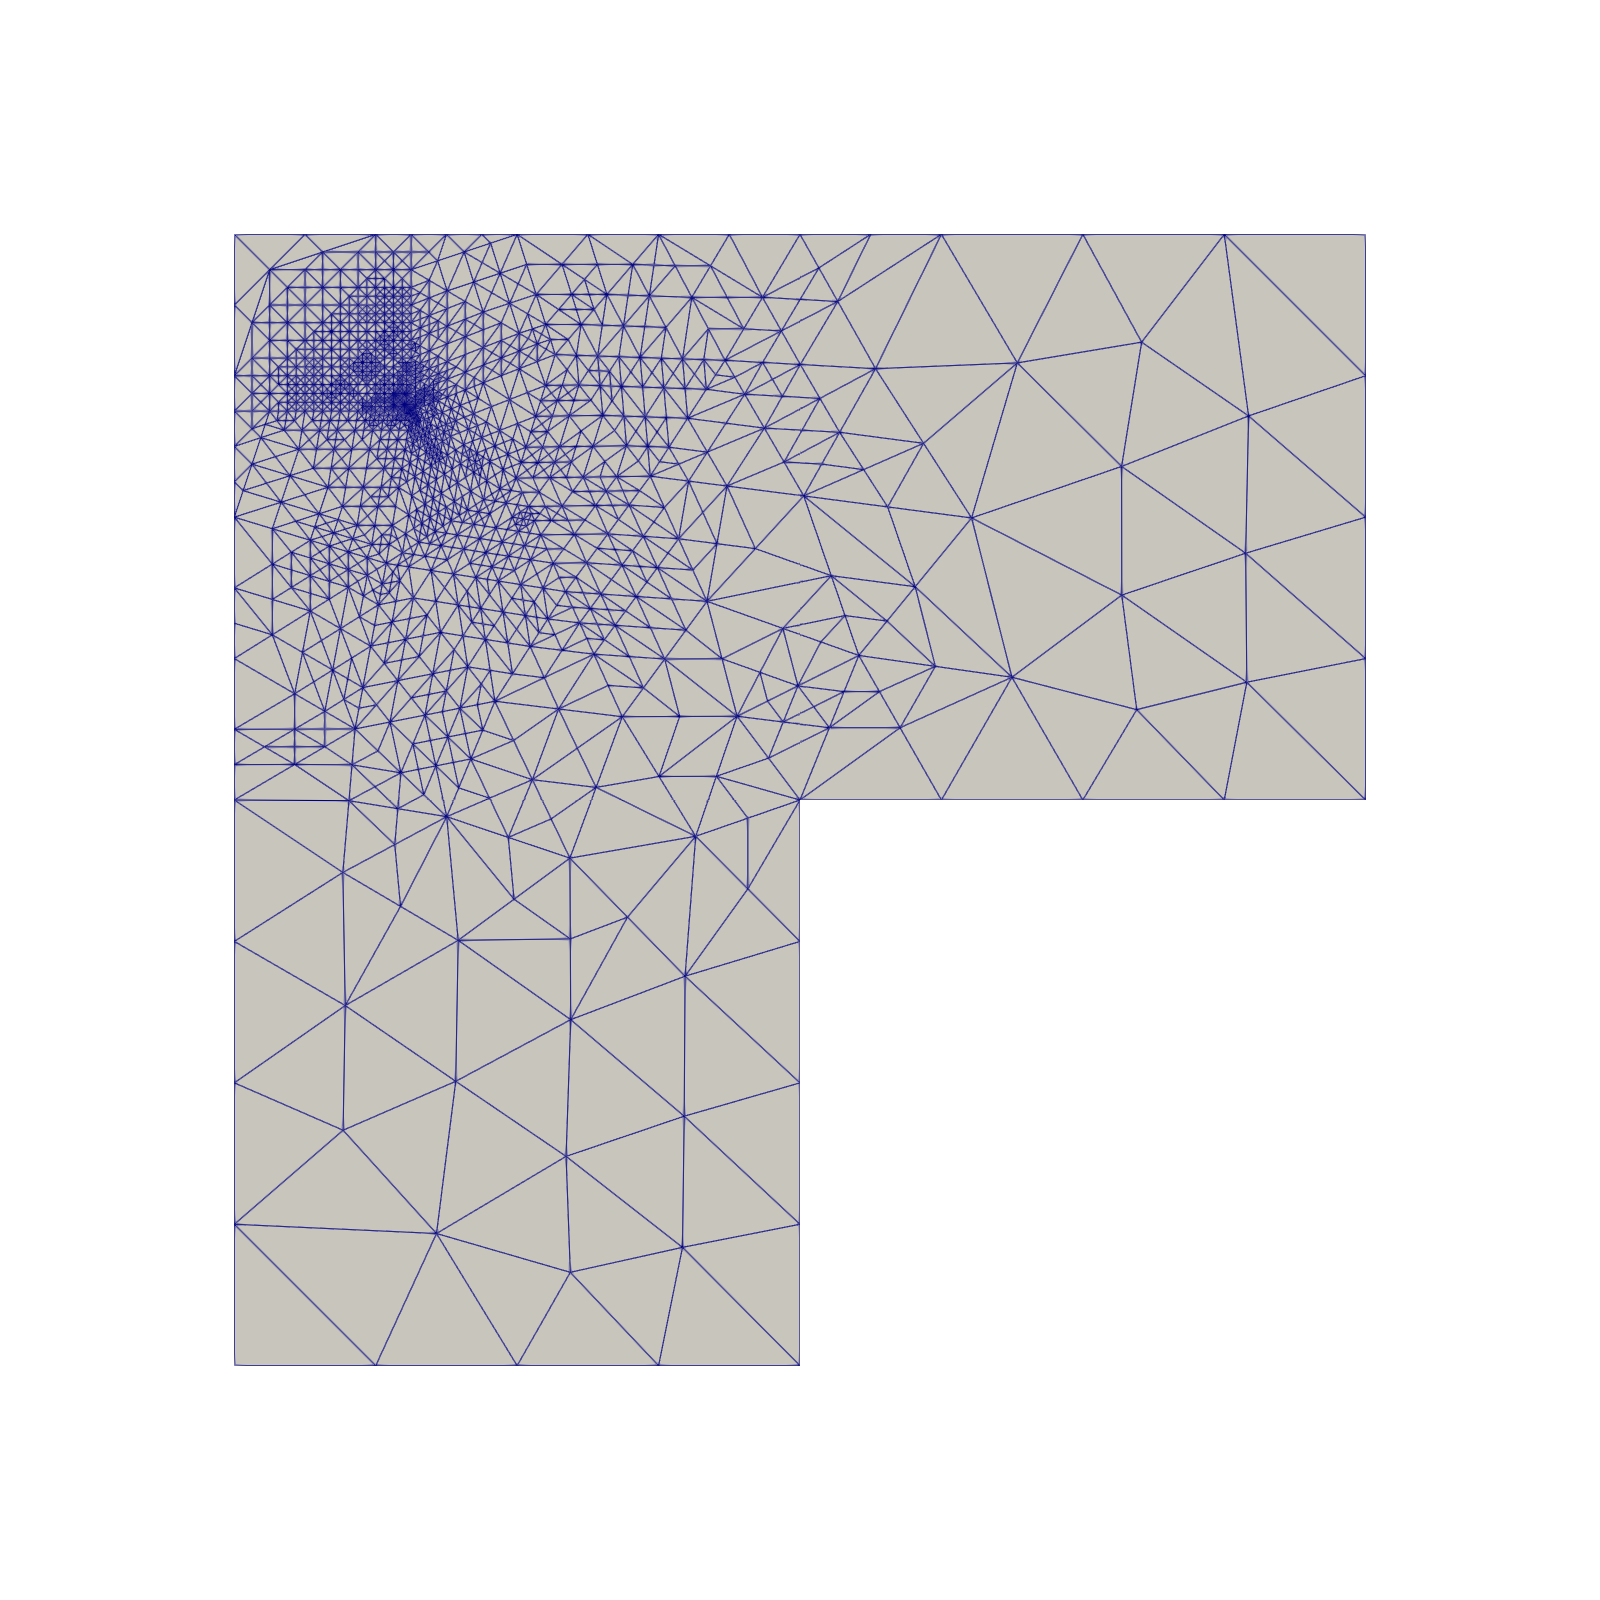
\includegraphics[
      width=\linewidth]{figures/lshape/j1_mesh.0003.png}
    \caption{}
  \end{subfigure}
  \hfill
  \begin{subfigure}[t]{0.31\textwidth}
    \centering
    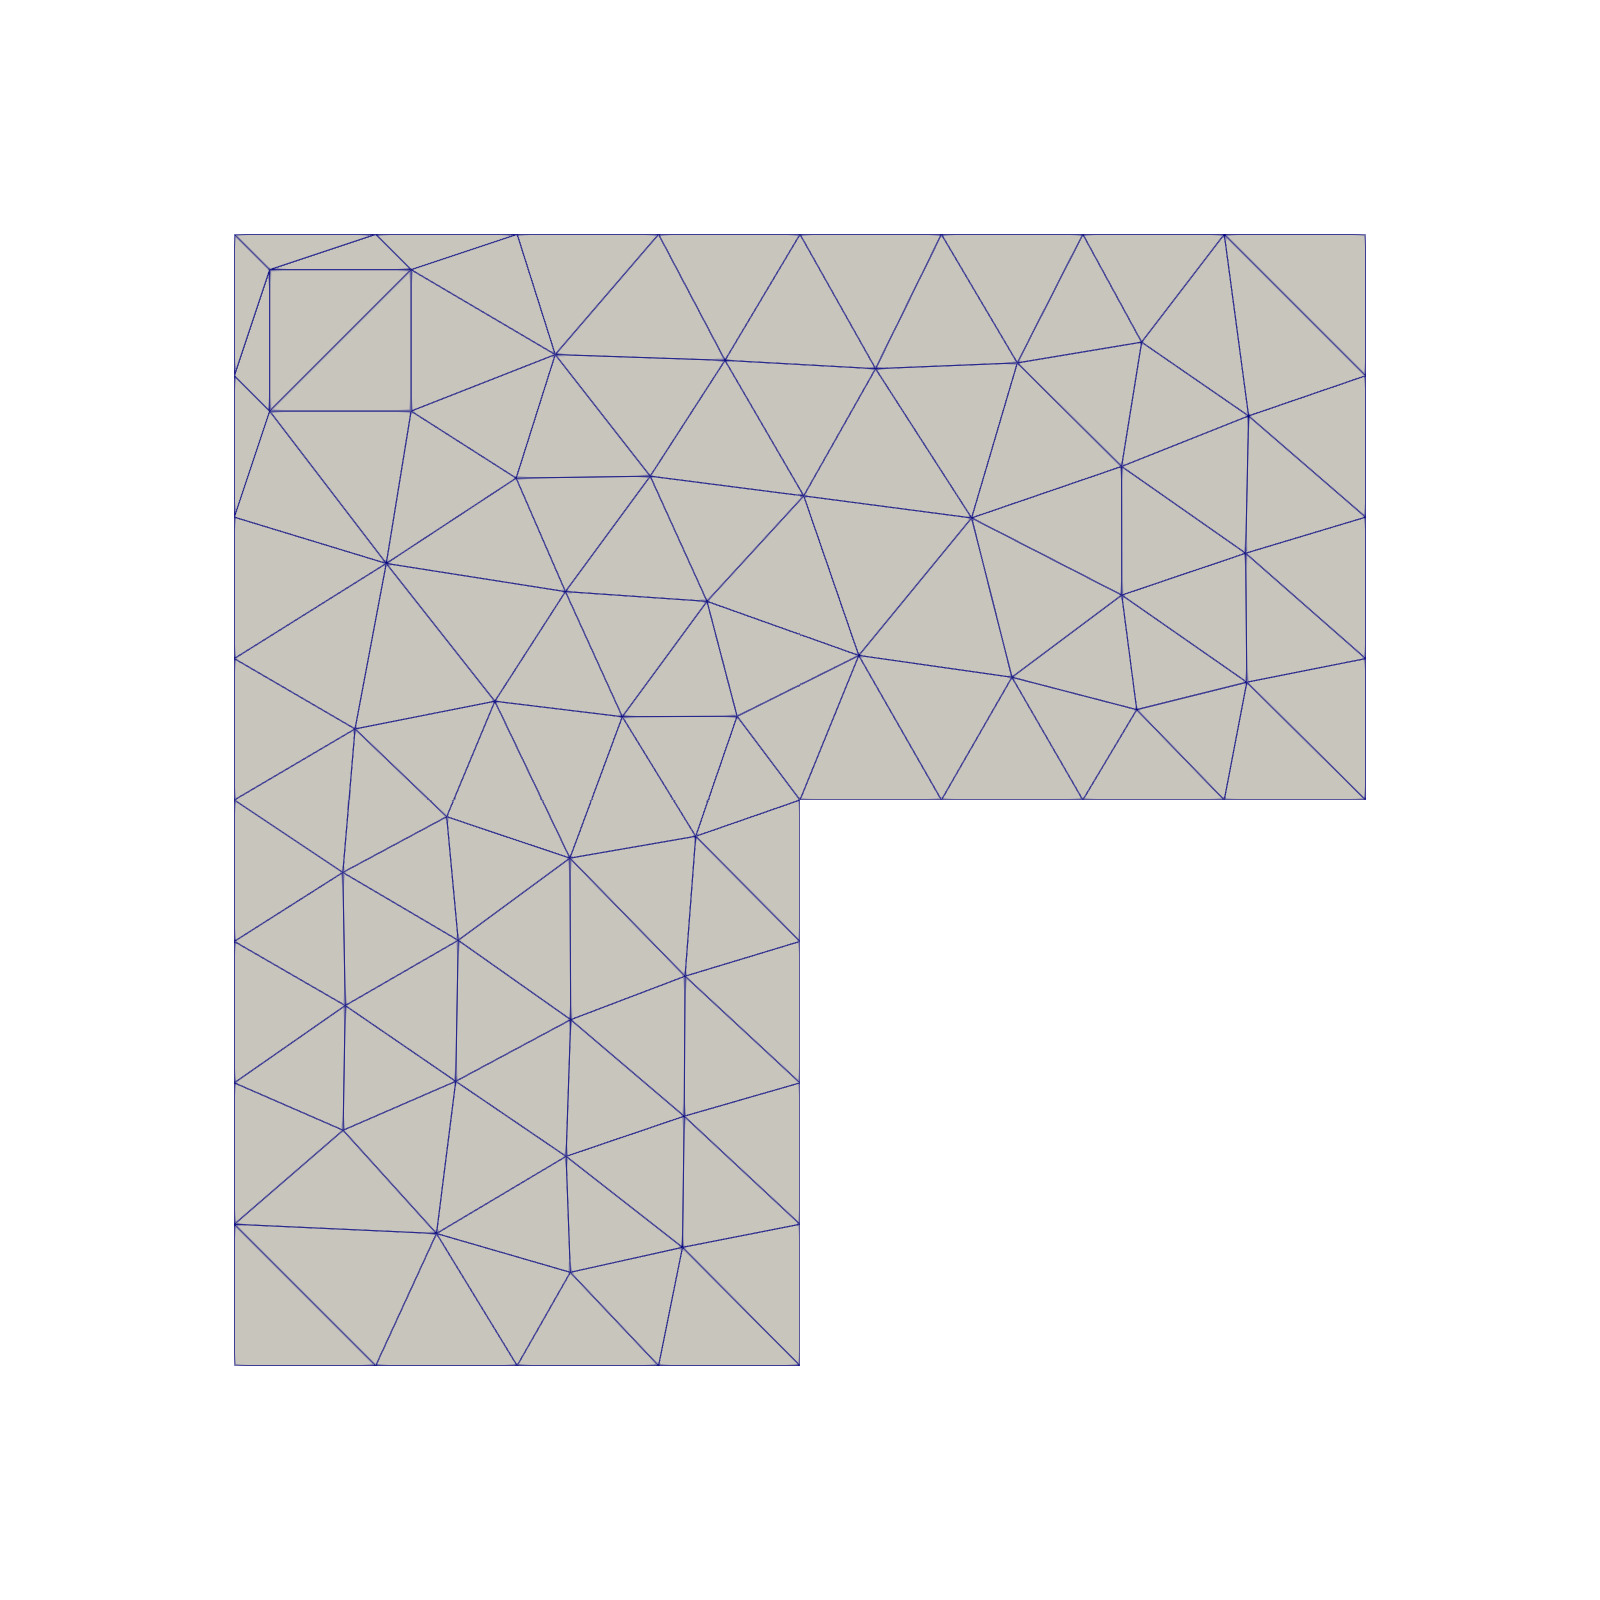
\includegraphics[
      width=\linewidth
    ]{figures/lshape/j1_mesh.0004.png}
    \caption{}
  \end{subfigure}
  \caption{Spatial meshes for goal $J_2$ at iteration~8. (a) shows the initial mesh, (b)--(e) show the spatial meshes carried by the adaptive time slabs whose right endpoints are $t=0.5$, $0.625$, $0.75$, and $1$, respectively.}
  \label{fig:lshape-j1-meshes}
\end{figure}
% \pef{I'm not sure this figure adds anything, I don't know how to interpret it.}

The mesh sequence clarifies the advantage of goal-oriented adaptivity. At $t=0.625$ and $t=0.75$, the selected slabs contain \(2\,176\) and \(3\,099\) cells, respectively, whereas the terminal slabs contain only the initial $116$ cells. Refinement is concentrated around $\Omega_I$ and its surrounding sensitivity region, and does not over-resolve the re-entrant corner. The DWR algorithm does not attempt to resolve every feature of the solution, only those that matter for the computation of the specified goal. DWR can be much more efficient than uniform refinement such as this.

